% =====================================================================
% Deciding What to Doubt - shortened submission version
% Advanced Topics in Mathematical Modelling
% University of Luxembourg, August 2026
% Compile: latexmk -pdf main_short.tex
% =====================================================================
\documentclass[12pt,a4paper]{article}

\usepackage[T1]{fontenc}
\usepackage[utf8]{inputenc}
\usepackage[sc]{mathpazo}
\usepackage[scaled=0.92]{helvet}
\usepackage{courier}
\usepackage{textcomp}
\usepackage{microtype}
\usepackage[top=2.6cm,bottom=2.6cm,left=2.5cm,right=2.5cm]{geometry}
\usepackage{amsmath,amssymb}
\usepackage{graphicx}
\usepackage{booktabs}
\usepackage{array}
\usepackage[round]{natbib}
\usepackage[font=small,labelfont={bf},skip=5pt]{caption}
\usepackage{setspace}
\usepackage[hidelinks]{hyperref}

\graphicspath{{figures/}{./}}
\linespread{1.05}
\setlength{\parskip}{4pt plus 1pt minus 1pt}
\setlength{\parindent}{1.3em}
\setlength{\tabcolsep}{4pt}

\newcommand{\work}[1]{\textit{#1}}

\begin{document}

% =====================================================================
% Title page
% =====================================================================
\begin{titlepage}
  \centering
  \vspace*{0.45cm}

  \IfFileExists{uni_logo.png}{%
    
\includegraphics[width=0.27\textwidth]{uni_logo.png}}{%
    \IfFileExists{figures/uni_logo.png}{%
      
\includegraphics[width=0.27\textwidth]{figures/uni_logo.png}}{%
      \vspace*{2.3cm}}}

  \vspace{0.8cm}
  {\normalsize\textsc{Faculty of Science, Technology and Medicine}\par}

  \vfill
  \rule{0.84\textwidth}{0.4pt}\par
  \vspace{0.75cm}
  {\LARGE\bfseries Deciding What to Doubt\par}
  \vspace{0.45cm}
  {\large\itshape How automated quality control for environmental\\
   sensor networks learned what to distrust\par}
  \vspace{0.75cm}
  \rule{0.84\textwidth}{0.4pt}\par

  \vfill
  {\normalsize Reading report submitted for the course\par}
  \vspace{0.2cm}
  {\normalsize\textsc{Advanced Topics in Mathematical Modelling}\par}
  \vspace{0.45cm}
  {\normalsize Master of Science in Mathematics\par}
  \vspace{0.75cm}
  {\normalsize Written alongside an internship at the Luxembourg Institute\\
   of Science and Technology, ENVISION unit\par}

  \vfill
  \begin{minipage}[t]{0.47\textwidth}
    \raggedright
    {\itshape Author:}\par
    Vaibhav Kailash MANGROLIYA\par
    \vspace{0.15cm}
    Matricule: 0246807154
  \end{minipage}%
  \hfill
  \begin{minipage}[t]{0.47\textwidth}
    \raggedleft
    {\itshape Academic supervisor:}\par
    Senthil Murugan NAGARAJAN\par
    \vspace{0.3cm}
    {\itshape Course responsible:}\par
    Jack S. HALE
  \end{minipage}

  \vspace{1.0cm}
  {\normalsize August 2026\par}
\end{titlepage}

% =====================================================================
% Front matter - kept compact on purpose
% =====================================================================
\thispagestyle{empty}
\section*{Summary}

Automated quality control (QC) decides whether a sensor reading should be
trusted, flagged, or reviewed. This report studies five works that shaped
that decision: Grubbs' classical outlier test, Iglewicz and Hoaglin's robust
modified z-score, the Oklahoma Mesonet QC system of Shafer and colleagues,
the general sensor-QC framework of Campbell and colleagues, and the
model-based comparison of Leigh and colleagues.

The report is organised around the five roles suggested by the course:
Historian, Technician, Experimentalist, Futurist and Critic. The main idea is
simple. Every QC method needs (1) a quantity that measures how unusual a
reading is, (2) a reference for what ``normal'' looks like, and (3) a
threshold that converts the score into a decision. The mathematics of the
score changes less than the reference and the threshold.

I test the main quantitative methods on a reproducible synthetic temperature
series with known faults. The experiments show three practical results. A
method can fail when its assumptions do not match time-series data; a single
threshold cannot remove that mismatch; and a small battery of simple checks
performs better than any one check alone. The report therefore argues for
transparent combinations of checks, explicit threshold justification, and
human review of flags rather than automatic deletion.

\subsection*{Use of Generative AI}
In accordance with the University of Luxembourg's AI guidelines, generative
AI (Claude, Anthropic) was used for text improvement, proofreading,
restructuring and iterative feedback. It was used as an editorial aid, not
to generate the substantive analysis, experimental results, or conclusions
from the bottom up. I have reviewed the report in full and can explain and
justify the work.

\subsection*{How this differs from my thesis}
My thesis documents a quality-control pipeline that I extended and audited
for an environmental monitoring network. This reading report instead studies
the literature behind such checks and uses a separate synthetic benchmark to
compare their behaviour. The aim, evidence and structure are therefore
different from the thesis.

\clearpage
\thispagestyle{empty}
\section*{Acknowledgments}

My thanks go first to my supervisor, \textbf{Dr. Senthil Murugan Nagarajan},
for his supervision and support throughout my Master's thesis. The questions
behind this report grew out of that broader work, especially the need to
understand why particular quality-control methods and thresholds are used.

I am grateful to \textbf{Dr. Jack S. Hale} for designing a course that asks
a student to read deeply rather than broadly. The Historian, Technician,
Experimentalist, Futurist and Critic roles provided a useful structure for
turning five readings into one argument.

I also thank the ENVISION unit at the Luxembourg Institute of Science and
Technology for the internship context that motivated these questions, and
the University of Luxembourg for the academic environment in which I could
pursue them.

\vspace{0.5cm}
\begin{spacing}{0.96}
\tableofcontents
\end{spacing}

\clearpage
\pagenumbering{arabic}

% =====================================================================
% 1. Introduction
% =====================================================================
\section{Introduction}
\label{sec:intro}

A weather station can produce thousands of readings per day. A network of
hundreds of stations produces more data than a person can inspect manually.
Yet those measurements feed flood warnings, climate records, research and
operational decisions. Somewhere between the sensor and the user, software
must decide which readings look trustworthy and which deserve attention.

That decision is harder than it first appears. A value may be physically
impossible, may jump too quickly, may stop changing, may disagree with a
neighbour, or may simply be an unusual but real event. A useful QC system
must detect faults without turning every rare event into an error. It must
also explain why it objected, because a flag is ultimately read by a person.

My interest in this problem came from an internship in which I extended and
audited an automated QC pipeline. The code contained familiar checks and
many configuration constants. That raised questions the code itself could
not answer: Why this statistic? Why this threshold? Which assumptions make
it valid? What happens when the same method is moved from an independent
sample to a correlated sensor stream?

This report answers those questions by reading five works in chronological
order and then testing the main quantitative ideas on a benchmark with known
faults. The five core readings are listed in Table~\ref{tab:fiveworks}.

\begin{table}[h]
\centering
\small
\caption{The five core readings and the role each plays in the report.}
\label{tab:fiveworks}
\begin{tabular}{@{}p{3.5cm}p{1.2cm}p{8.7cm}@{}}
\toprule
Work & Year & Why it matters \\
\midrule
\citet{grubbs1969} & 1969 & Classical hypothesis-test view of an outlying observation. \\
\citet{iglewicz1993} & 1993 & Robust modified z-score using the median and MAD; source of the 3.5 screening rule. \\
\citet{shafer2000} & 2000 & A complete operational QC system for a large automatic weather network. \\
\citet{campbell2013} & 2013 & General framework for QA/QC in streaming environmental sensor data. \\
\citet{leigh2019} & 2019 & Comparison of rule-based, regression and feature-based anomaly detection on labelled water-quality data. \\
\bottomrule
\end{tabular}
\end{table}

The course suggests five roles: Historian, Technician, Experimentalist,
Futurist and Critic. I use one section for each role. This keeps the report
close to the course structure and makes the main argument easy to follow.

% =====================================================================
% 2. Historian
% =====================================================================

\section{Historian: where the ideas came from}
\label{sec:history}

The history of QC can be read as a change in what counts as a reference for
``normal'' data.

Early outlier work treated the problem as a statistical test. By the middle
of the twentieth century, Grubbs collected practical procedures for deciding
whether one or more observations were too extreme to belong to a normally
distributed sample \citep{grubbs1969}. The attraction was clear: the method
gave a named statistic, a significance level and a defensible rule.

The weakness was also clear. Classical tests use the sample mean and standard
deviation, both of which are affected by the very outliers they are meant to
detect. Pearson and Chandra Sekar described the masking problem, where two
similar outliers inflate the standard deviation enough to hide each other
\citep{pearson1936}. Rosner later developed the generalised ESD procedure to
handle several possible outliers without stopping at the first insignificant
step \citep{rosner1983}.

Robust statistics changed the reference. Instead of estimating the centre
and spread with quantities that a few bad values can move strongly, robust
methods use the median and the median absolute deviation (MAD). Iglewicz and
Hoaglin turned that idea into a simple engineering rule: compute a modified
z-score and flag large values, commonly using 3.5 as a screening threshold
\citep{iglewicz1993}. This was designed for batches of observations, not for
a short moving window over a correlated stream, which becomes important in
Section~\ref{sec:experiment}.

The next change was operational. The Oklahoma Mesonet made QC a system rather
than a single test. Its design combined calibration, maintenance, automatic
checks, graded flags and human review \citep{shafer2000}. The important idea
was not a new equation. It was that reliable data quality comes from several
independent kinds of evidence and a process for acting on the flags.

Campbell and colleagues generalised this approach for streaming
environmental sensors \citep{campbell2013}. They separate quality assurance
(what is done before data collection) from quality control (what is done to
the data afterwards), distinguish faults from real anomalies, and argue for
preserving raw values together with QC flags.

Leigh and colleagues then returned to explicit statistical comparison. On
high-frequency water-quality data they compared rule-based, regression-based
and feature-based methods and reported performance by fault type
\citep{leigh2019}. Their result is important for this report: no method wins
for every fault, so combinations are more useful than a search for one
universal detector.

\begin{figure}[h]
  \centering
  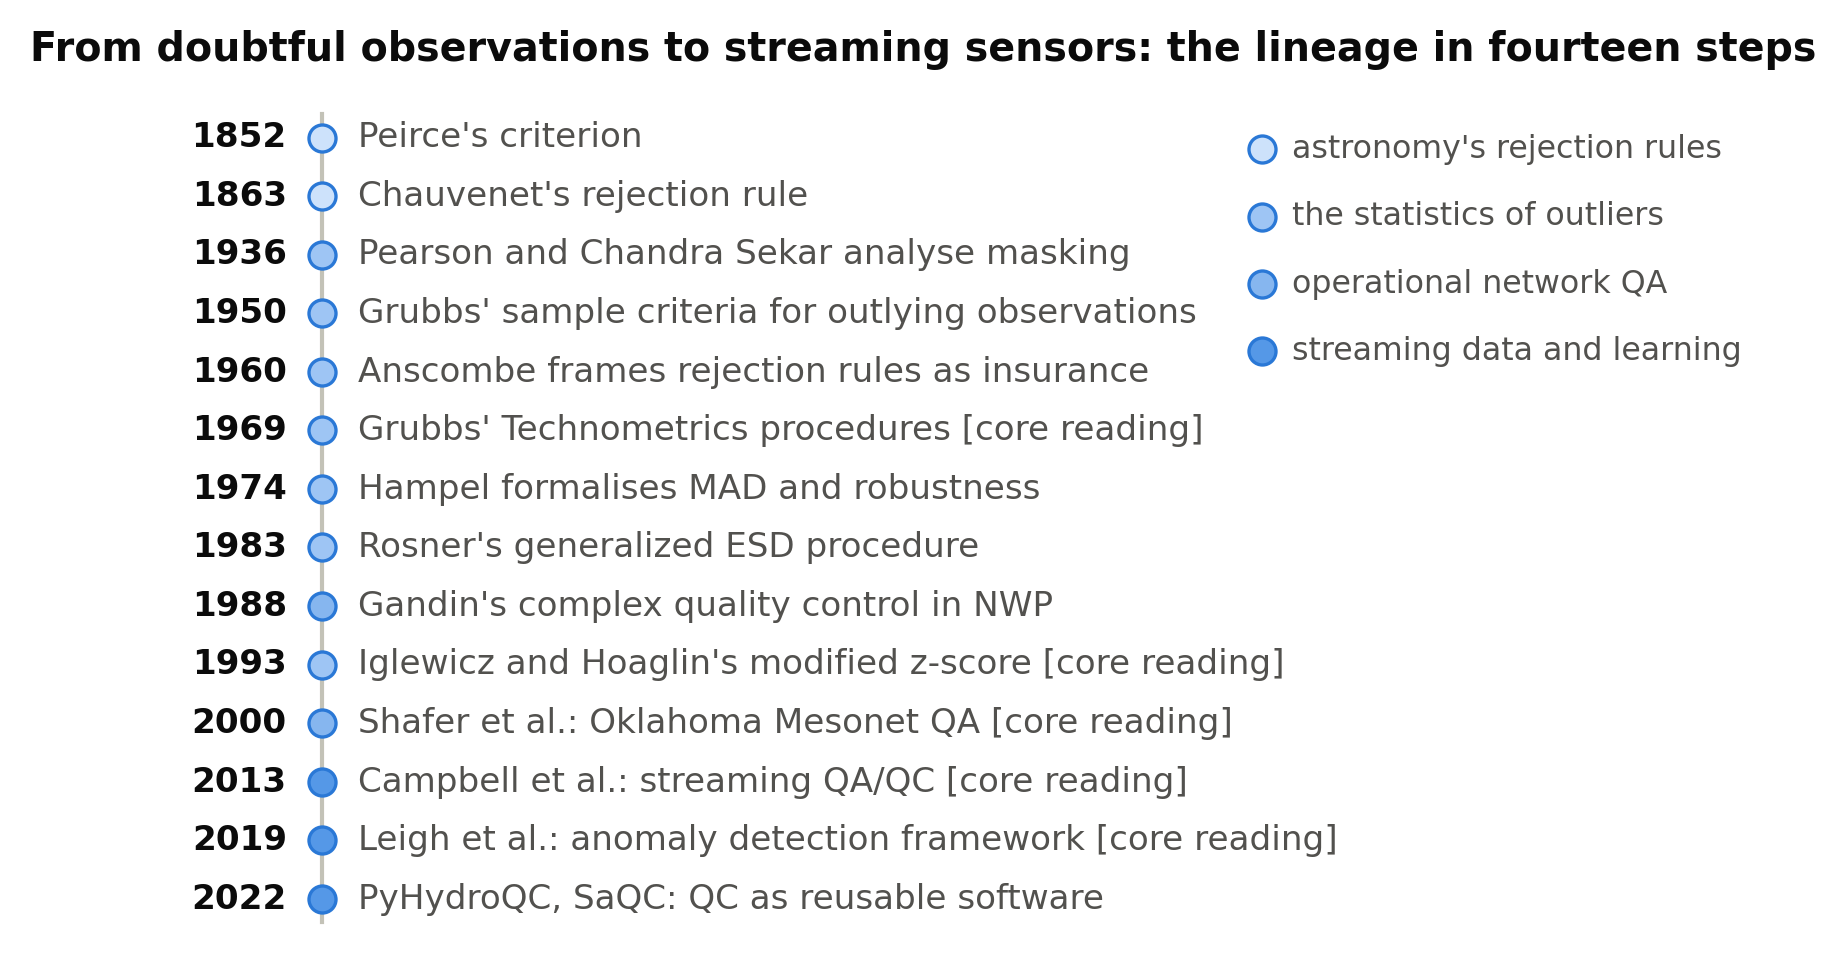
\includegraphics[width=0.93\textwidth]{fig_timeline.png}
  \caption{A compact timeline of the line followed in this report. The five
  core readings are marked in the labels.}
  \label{fig:timeline}
\end{figure}

The historical pattern is therefore simple. The score used to measure
surprise changed slowly. The reference for normality moved from theoretical
distributions, to robust summaries of the data, to engineering knowledge,
neighbouring stations and fitted models. The threshold remained the part
most likely to be inherited without enough justification.

% =====================================================================
% 3. Technician
% =====================================================================

\clearpage
\section{Technician: how the methods work}
\label{sec:methods}

\subsection{One idea behind the methods}

For a batch of readings $x_1,\ldots,x_n$, let $\bar{x}$ be the mean, $s$ the
standard deviation, $\tilde{x}$ the median, and
\[
\mathrm{MAD}=\operatorname{median}_i |x_i-\tilde{x}|.
\]
For a time series, $x_t$ denotes the value at time $t$.

Most methods in this report can be described by three parts:

\begin{enumerate}
  \item a \textbf{score} that says how unusual a reading is;
  \item a \textbf{reference} that describes normal behaviour;
  \item a \textbf{threshold} that converts the score into a flag.
\end{enumerate}

Keeping these parts separate is useful. A method can have a sensible score
but a poor reference, or a good reference but an unsuitable threshold.

\subsection{Classical and robust outlier scores}

Grubbs' statistic for the most extreme observation is
\begin{equation}
G=\frac{\max_i |x_i-\bar{x}|}{s}.
\label{eq:grubbs}
\end{equation}
The null hypothesis is that all observations come from one normal
population. A critical value is calculated from the sample size and chosen
significance level \citep{grubbs1969}. This is appropriate when the sample
matches the assumptions. A sensor stream with a daily cycle and strong
temporal correlation does not look like one independent normal batch.

The modified z-score replaces the fragile mean and standard deviation by the
median and MAD:
\begin{equation}
M_i=\frac{0.6745(x_i-\tilde{x})}{\mathrm{MAD}}.
\label{eq:modz}
\end{equation}
Iglewicz and Hoaglin recommend flagging observations with
$|M_i|>3.5$ as a practical screening rule \citep{iglewicz1993}. The score is
robust to a few extreme values, but the behaviour still depends on which
observations are placed in the window and on the threshold used.

\subsection{Operational checks}

Automatic environmental QC normally uses several simple checks rather than
one statistical test. Table~\ref{tab:checks} gives the small set used in this
report.

\begin{table}[h]
\centering
\small
\caption{The main checks, what they ask, and their main limitation.}
\label{tab:checks}
\begin{tabular}{@{}p{2.7cm}p{5.2cm}p{6.0cm}@{}}
\toprule
Check & Basic question & Main limitation \\
\midrule
Range & Is the value physically or instrumentally possible? & Cannot see plausible but wrong values. \\
Step & Did the value change more than a chosen amount between samples? & Misses slow drift and small level shifts. \\
Persistence & Has the sensor stopped changing? & Exact equality misses a stuck sensor with small last-digit jitter. \\
Internal consistency & Do related quantities at one station obey physical relationships? & Shows a contradiction but not necessarily which sensor is wrong. \\
Spatial consistency & Does the station agree with nearby stations after normal offsets are allowed for? & Can flag real local weather; depends on having suitable neighbours. \\
Outlier score & Is the reading unusual relative to a batch or moving window? & Depends strongly on the reference window and its assumptions. \\
Forecast & Is the reading far from what recent history predicted? & One-step forecasts often absorb slow drift and persistent faults. \\
\bottomrule
\end{tabular}
\end{table}

The checks should be read as different kinds of evidence. A range check uses
instrument knowledge. A step or persistence check uses the recent behaviour
of the same series. Internal consistency uses physics. Spatial consistency
uses redundancy across stations. Forecasting uses a fitted model of the
past. Their weaknesses are different, which is exactly why a battery can be
stronger than one check.

\subsection{Persistence as a useful example}

A stuck sensor can be tested in two ways. The simple implementation looks
for an exact run of repeated values:
\begin{equation}
\text{flag if }x_t\text{ belongs to a run of at least }n_{\mathrm{run}}
\text{ identical values.}
\end{equation}
A more robust version looks for a collapse in variability:
\begin{equation}
\text{flag window }W_t\iff \operatorname{sd}\{x_u:u\in W_t\}<s_{\min}.
\end{equation}
The second form is closer to the operational idea in \citet{shafer2000}.
It catches both a perfectly frozen value and a sensor that remains stuck but
jitters slightly in the last digit. This small example illustrates a wider
lesson: the exact definition of a check matters as much as its name.

\subsection{How a QC system should use the verdicts}

A useful QC pipeline should keep the original measurement and attach a
verdict or quality code rather than silently overwrite the data. A failed
range check may make a value unusable for later calculations, but the value
and the reason for rejecting it should remain auditable. Other checks usually
produce flags for later review because disagreement may represent either a
fault or a real event \citep{shafer2000,campbell2013}.

The order can also matter. Cheap checks can run before expensive spatial or
model-based checks, and clearly invalid values should not be used as evidence
for later checks. The important principle is transparency: the user should
be able to tell which check objected and why.


\subsection{The checks in plain language}

The table above is useful as a summary, but the checks are easier to explain
with one simple example each. I keep the descriptions here deliberately
practical, because these are the questions I would use when explaining the
system to an operator or to a reviewer.

\paragraph{Range check.}
Suppose an air-temperature sensor reports $-999$\,\textcelsius. The number
is not merely unusual; it is outside the operating range of the sensor and
outside any realistic environmental range. A range check compares the value
with a lower and upper limit and flags it immediately. This check is cheap
and easy to defend. Its weakness is that most real faults remain inside
plausible limits. A sensor that is wrong by 2\,K may still pass perfectly.

\paragraph{Step check.}
A step check asks whether two consecutive readings differ by more than a
chosen limit. For five-minute temperature data, a sudden jump of several
kelvin may be suspicious. This is good for spikes and abrupt failures. It is
not good for slow problems. A sensor that drifts by a tiny amount at every
sample can become badly wrong while never making one large step.

\paragraph{Persistence check.}
A persistence check looks for a sensor that has stopped responding. The
simplest version searches for exactly repeated values. That works if the
instrument sends the same number again and again. A more realistic faulty
sensor may still move in its last digit, so a low-variability version is
safer: instead of asking whether all values are identical, it asks whether
the variation inside a window has become abnormally small.

\paragraph{Internal-consistency check.}
Some quantities are related by physics. Dew-point temperature should not
normally exceed air temperature, and daily minimum temperature should not be
higher than daily maximum temperature. When two related quantities break a
physical relationship, at least one reading deserves attention. The limit
of the check is that it can show a contradiction without always identifying
which sensor caused it.

\paragraph{Spatial-consistency check.}
Nearby stations provide an external reference. If one station suddenly moves
away from several healthy neighbours while the neighbours continue to agree,
the station is suspicious. This is particularly useful for level shifts,
stuck sensors and drift. However, local weather can be real. A thunderstorm
may affect one station and not another, so disagreement is evidence for
review, not proof that a sensor is wrong.

\paragraph{Outlier-score check.}
An outlier score asks how far a reading lies from the centre of a reference
set. Grubbs uses the mean and standard deviation; the modified z-score uses
the median and MAD. These scores are useful only when the reference set makes
sense. A whole month of temperature contains a daily cycle, while a very
short window may be noisy. The main design question is therefore not only
``which score?'' but also ``which observations define normal?''

\paragraph{Forecast check.}
A forecast method predicts the next reading from recent history and flags a
large prediction error. A sudden spike is difficult to predict and therefore
easy to flag. Slow drift is different: if the model keeps updating from the
recent past, it can follow the drifting sensor and stop being surprised. The
method is therefore useful evidence for sudden changes, not a complete
solution to every fault.

These seven checks can be grouped into three simple sources of evidence.
Range and internal-consistency checks use physical knowledge. Step,
persistence, outlier and forecast checks use the behaviour of the same time
series. Spatial checking uses other stations. A strong QC system combines
these sources rather than asking one source to do everything.

\subsection{A simple running example}

Consider one station reporting air temperature every five minutes. At
10:00 it reports 12.1\,\textcelsius, at 10:05 it reports
12.2\,\textcelsius, and at 10:10 it reports 18.5\,\textcelsius. A range check
may accept all three values because 18.5\,\textcelsius is physically
possible. A step check may flag 10:10 because the jump is too large. A
rolling outlier score may also flag it because it is far from the recent
window. If neighbouring stations remain around 12\,\textcelsius, the spatial
check adds independent evidence that the value is suspicious.

Now consider a different failure. The sensor begins at 12.0\,\textcelsius
and then reports 12.01, 12.00, 12.02 and 12.01 for several hours while the
real temperature changes normally. The range check passes it and the step
check sees nothing unusual. Exact repetition may also miss it because the
values are not identical. A low-variability persistence check can detect the
collapse in movement, and the spatial check can detect the growing
disagreement with neighbouring stations.

These two examples explain why the pipeline needs several checks. The first
fault is sudden and visible in the local series. The second fault remains
plausible and requires a different definition of persistence or an external
reference. The checks are therefore complementary rather than competing.

% =====================================================================
% 4. Experimentalist
% =====================================================================

\clearpage
\section{Experimentalist: testing the methods}
\label{sec:experiment}

\subsection{Benchmark design}

Real sensor archives rarely provide a certain answer about every reading. To
compare methods directly, I built a synthetic month of air temperature with
30 days of five-minute samples, giving 8640 readings. The clean signal
contains a daily cycle, a slower weather component and correlated sensor
noise. I then inserted five fault types based on the fault categories
discussed by \citet{campbell2013} and \citet{leigh2019}:

\begin{itemize}
  \item 14 sudden spikes between 3 and 8 K;
  \item a $+2.5$ K level shift lasting 36 hours;
  \item a frozen sensor for 6 hours with exact repetition;
  \item a frozen sensor for 6 hours with $\pm0.02$ K jitter;
  \item a slow calibration drift reaching $+2.2$ K over four days.
\end{itemize}

Three healthy neighbouring stations share the same broad weather pattern but
have their own offsets and noise. Random-number generators are seeded, so the
benchmark and figures are exactly reproducible.

\begin{figure}[h]
  \centering
  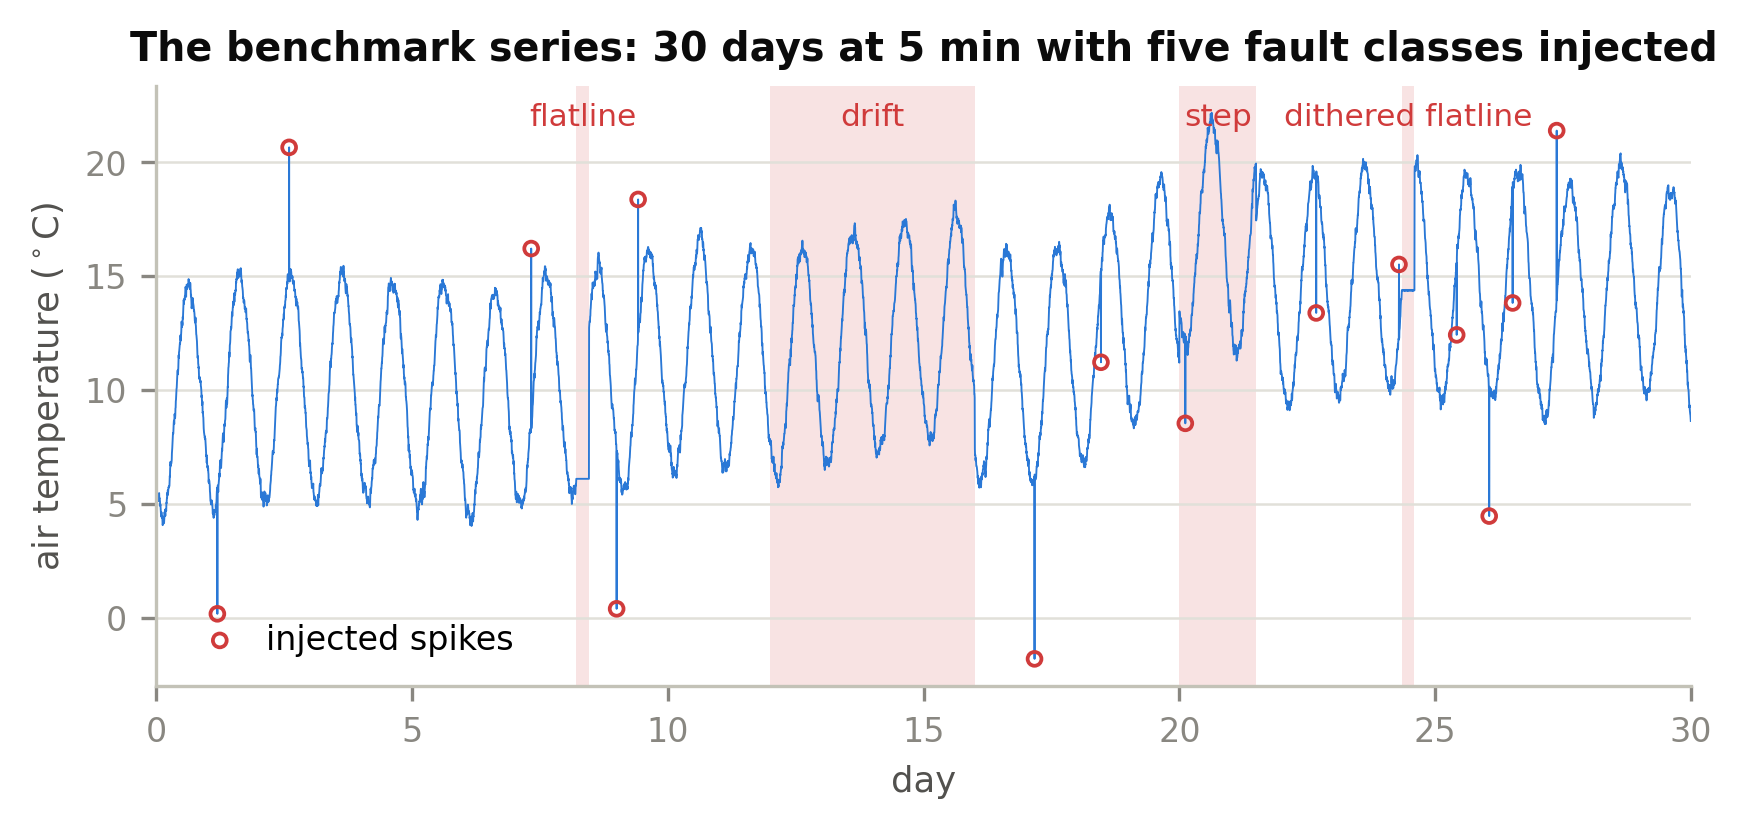
\includegraphics[width=0.95\textwidth]{fig_series.png}
  \caption{Synthetic temperature benchmark. Shaded regions are segment
  faults; circles mark the injected spikes.}
  \label{fig:series}
\end{figure}

For spikes, I count a fault as detected if a flag falls within one sample of
the injected spike. For segment faults, I report the percentage of faulty
readings flagged. False alarms are flags on clean readings and are reported
per day for one series.

\subsection{Masking: why a classical test can miss two outliers}

I first reproduced the masking problem. Eighteen values were placed tightly
around 10.0 and two equal outliers at 10.6 were added. The pair increases the
sample standard deviation enough that the largest Grubbs statistic is about
2.56, below the critical value of about 2.71 for this sample. An iterated
single-outlier Grubbs procedure therefore stops and finds nothing. Rosner's
generalised ESD, which evaluates several possible removals before deciding,
finds the two outliers \citep{rosner1983}.

\begin{figure}[h]
  \centering
  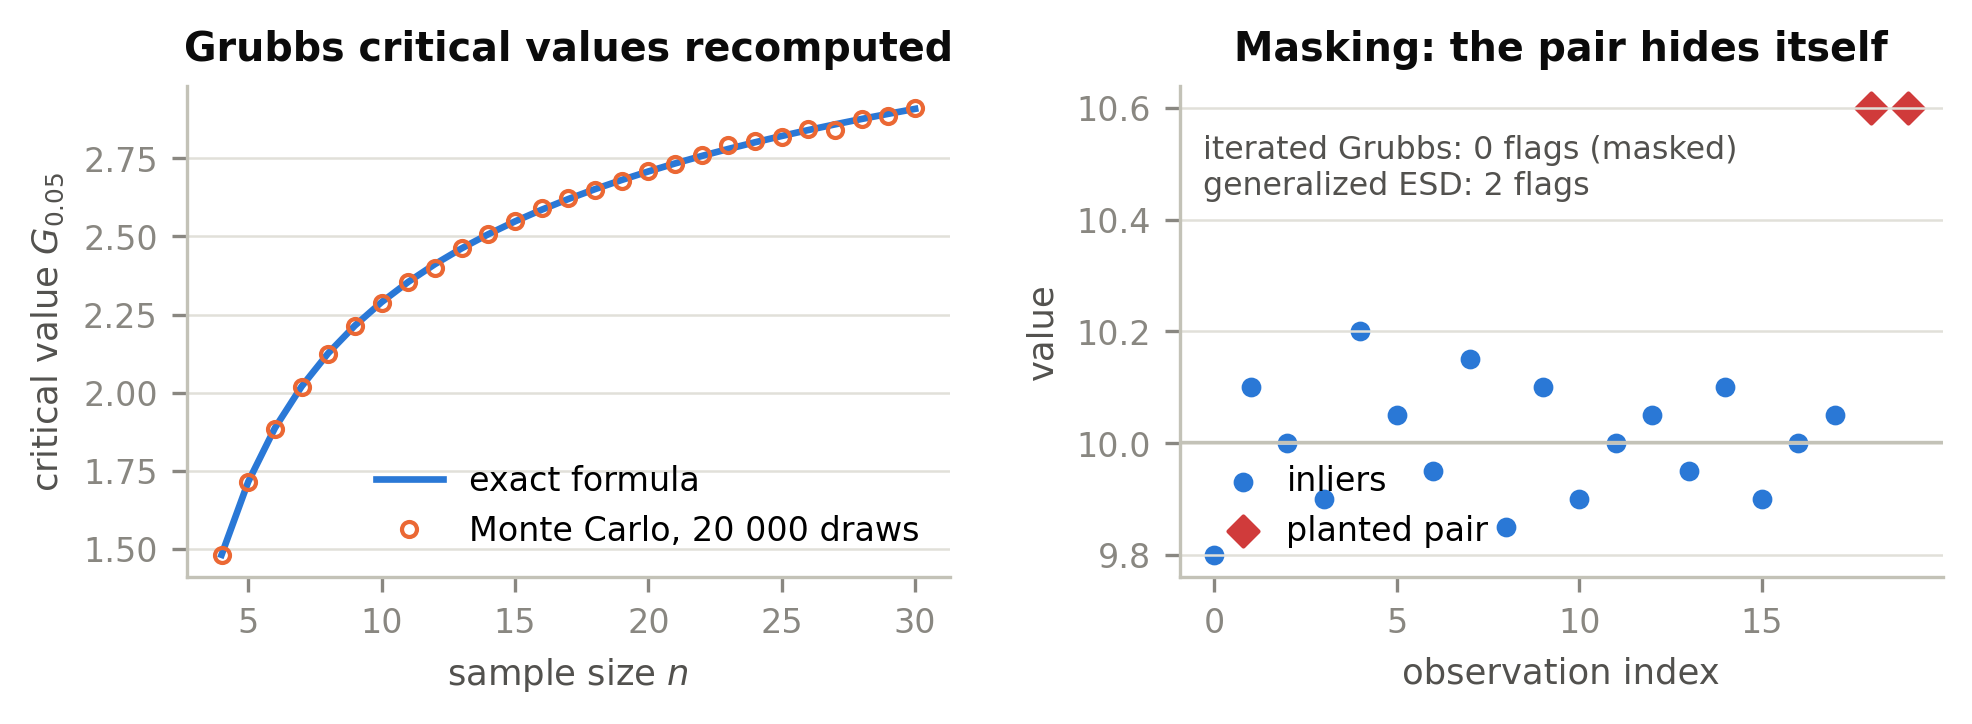
\includegraphics[width=0.92\textwidth]{fig_grubbs.png}
  \caption{Left: Grubbs critical values checked by simulation. Right: the
  masking example, where a pair defeats the iterated single-outlier test but
  generalised ESD finds both.}
  \label{fig:grubbs}
\end{figure}

This experiment is useful because the failure comes from the reference
statistics, not from complicated data. Two bad values can change the
standard deviation used to judge themselves.

\subsection{The modified z-score: a good statistic with a context problem}

On the same small contaminated sample, the robust modified z-score separates
the two planted outliers because the median and MAD barely move. In that
setting, the method behaves as intended.

The problem appears when the same score is used in a short moving window over
a correlated sensor stream. I tested windows of 7, 25 and 97 samples and
swept the threshold from 2 to 400. At a 7-sample window, the textbook value
3.5 detects all injected spikes but produces 1.63 false alarms per day for a
single series. A threshold of 30 removes those false alarms but catches only
9 of the 14 spikes.

\begin{figure}[h]
  \centering
  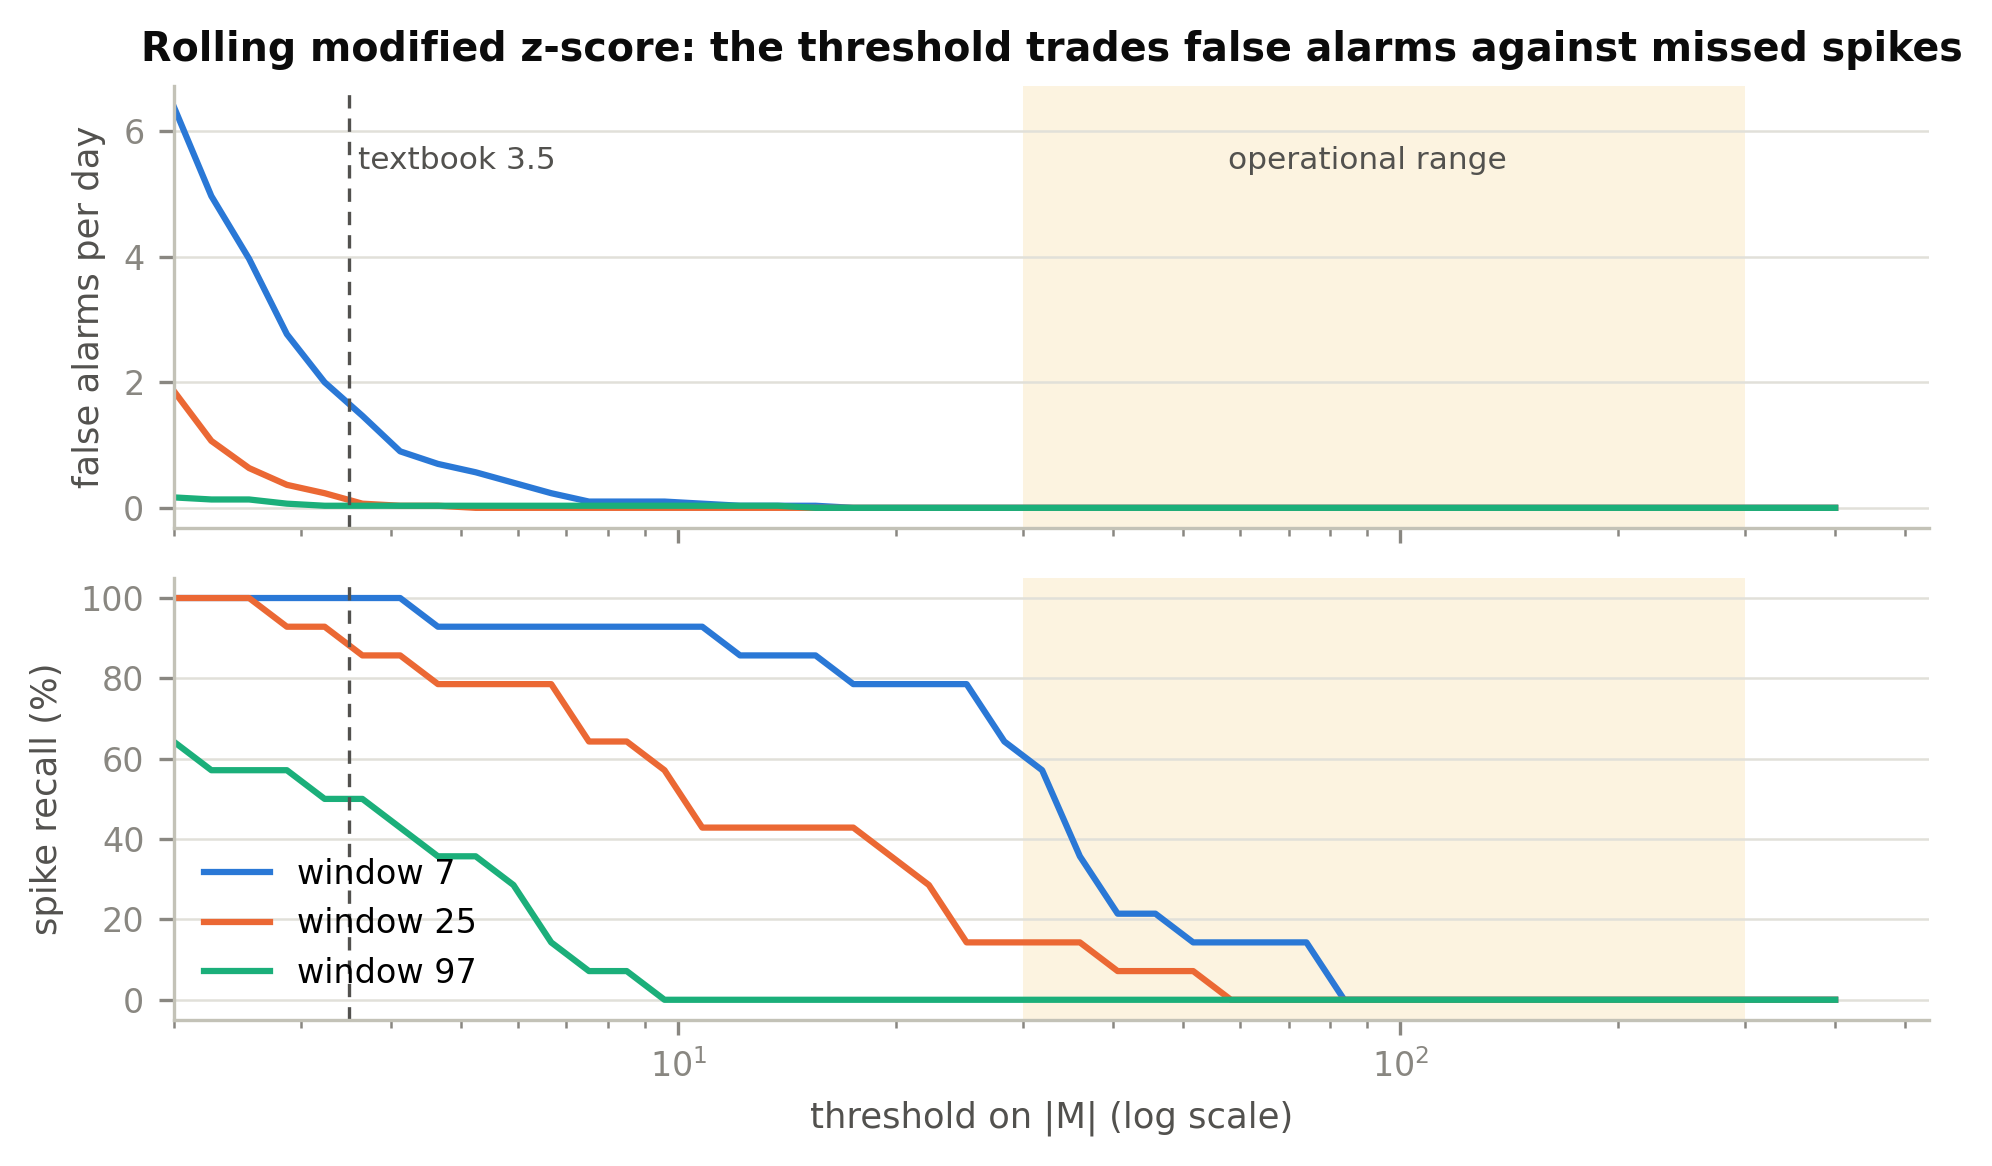
\includegraphics[width=0.92\textwidth]{fig_thresholds.png}
  \caption{False alarms and spike detection as the modified z-score
  threshold changes. The dashed line is 3.5. No threshold is both silent and
  complete for the tested windows.}
  \label{fig:thresholds}
\end{figure}

The important point is not that 3.5 is ``wrong'' or 30 is ``right''. The
point is that a threshold calibrated for one data setting should not be
copied into another without measuring what it costs. Window length, sampling
rate, noise and threshold form one design problem.

\subsection{Comparing the checks}

I then ran the main implementable checks over the same benchmark. Internal
consistency is not scored because the benchmark has only one measured
quantity per station. The feature-based branch from \citet{talagala2019} is
also not implemented because fourteen events are too few for a meaningful
evaluation of its extreme-value machinery.

Table~\ref{tab:results} gives the exact comparison. The final row is a simple
battery that takes the union of the step, variance-persistence and spatial
checks.

\begin{table}[h]
\centering
\small
\setlength{\tabcolsep}{2.8pt}
\caption{Percentage of faulty readings flagged, with false alarms per day.}
\label{tab:results}
\begin{tabular}{@{}lrrrrrr@{}}
\toprule
Check & Spike & Shift & Exact & Jitter & Drift & False/day \\
\midrule
Range & 0.0 & 0.0 & 0.0 & 0.0 & 0.0 & 0.00 \\
Grubbs, whole month & 0.0 & 0.0 & 0.0 & 0.0 & 0.0 & 0.00 \\
Modified z, whole month, 3.5 & 0.0 & 0.0 & 0.0 & 0.0 & 0.0 & 0.00 \\
Modified z, win. 7, 3.5 & 100.0 & 0.9 & 0.0 & 2.8 & 1.0 & 1.63 \\
Modified z, win. 7, 30 & 64.3 & 0.2 & 0.0 & 0.0 & 0.0 & 0.00 \\
Step, 3 K/5 min & 100.0 & 0.5 & 0.0 & 0.0 & 0.0 & 0.50 \\
Persistence, exact & 0.0 & 0.0 & 100.0 & 0.0 & 0.0 & 0.00 \\
Persistence, variance & 0.0 & 0.0 & 100.0 & 100.0 & 0.0 & 0.00 \\
Spatial, neighbours & 100.0 & 99.8 & 80.6 & 81.9 & 32.4 & 0.10 \\
Forecast, one-step & 100.0 & 0.7 & 0.0 & 0.0 & 0.0 & 0.57 \\
\textbf{Battery: step + persist. + spatial} & \textbf{100.0} & \textbf{100.0} & \textbf{100.0} & \textbf{100.0} & \textbf{32.4} & \textbf{0.60} \\
\bottomrule
\end{tabular}
\end{table}

\begin{figure}[h]
  \centering
  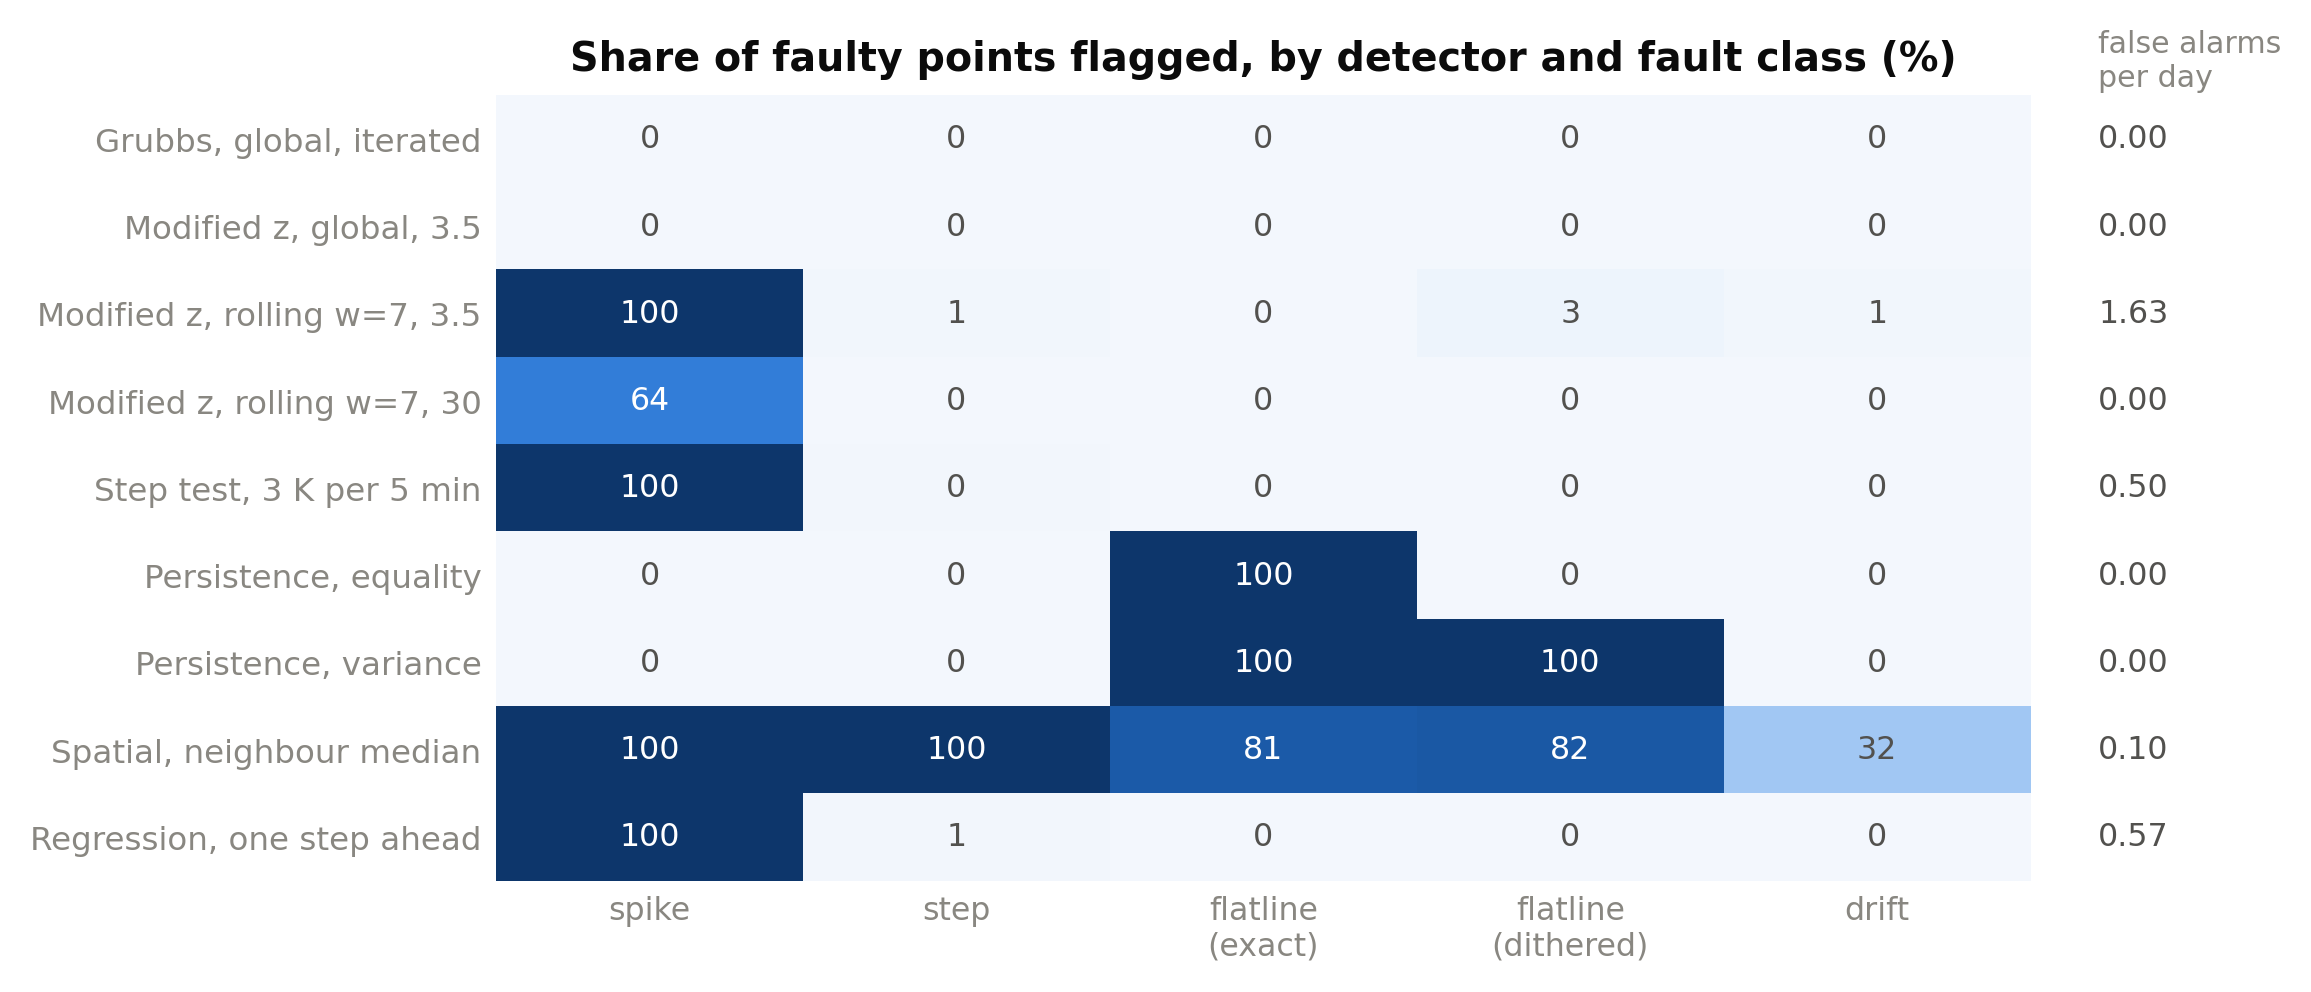
\includegraphics[width=0.95\textwidth]{fig_detectors.png}
  \caption{The same comparison as a detection matrix. No single check covers
  all fault types; the battery covers the first four completely and retains
  the spatial check's partial sensitivity to drift.}
  \label{fig:detectors}
\end{figure}

The results are easier to understand by fault type than by method. Spikes
are easy for step, rolling outlier and forecast checks. Exact persistence is
perfect for a perfectly frozen sensor but fails completely when the stuck
value jitters. The low-variability persistence check fixes that problem.
Spatial comparison is the strongest single detector because healthy
neighbours provide an external reference. Slow drift remains difficult and
is detected only after the accumulated difference becomes large enough.

The battery is the practical result I take most seriously. Three simple and
explainable checks cover more faults than any individual method. This agrees
with the operational philosophy of \citet{shafer2000} and the combination
recommended by \citet{leigh2019}.

\subsection{Limits of the experiment}

The benchmark is deliberately cleaner than the real world. It contains no
missing data, fouling that resembles natural behaviour, or local storms that
make one healthy station disagree with its neighbours. The neighbouring
stations are also more cooperative than real stations separated by complex
terrain. Therefore the exact percentages are properties of this benchmark,
not universal performance claims.

The constants are also chosen deliberately rather than derived: a 3 K step
limit, a 0.02 K variability floor, a three-standard-deviation spatial band,
and a wider forecast band. This is not hidden because it is part of the
point. A threshold is an engineering choice unless its assumptions and cost
have been demonstrated for the deployment.


\subsection{Reading the results by fault type}

The result table is easier to remember when it is read by fault rather than
by algorithm. This also matches the practical question an operator has:
``if this kind of sensor problem happens, which evidence is likely to find
it?''

\paragraph{Spikes.}
Spikes are the easiest fault in the benchmark. The step check catches all of
them because a spike creates an abrupt change. The rolling modified z-score
at threshold 3.5 and the one-step forecast also catch all of them. Spatial
comparison catches them because the neighbours remain healthy. This is a
good example of several independent checks agreeing on the same event.
Agreement does not make the value mathematically impossible, but it gives a
reviewer much stronger evidence than one flag alone.

\paragraph{Level shift.}
The planted level shift is $+2.5$\,K while the step limit is 3\,K per five
minutes. For that reason the step check is almost blind to it. The forecast
check notices mainly the entry to the new level and then adapts. Spatial
comparison performs much better because the target station stays separated
from the healthy neighbours for the duration of the fault. This illustrates
the value of an external reference: the station's own recent history may
accept a new level that its neighbours show to be suspicious.

\paragraph{Frozen sensor with exact repetition.}
Exact persistence is designed for this case and detects it completely. The
variance form also detects it because a perfectly repeated value has zero
spread. Spatial comparison detects most of the period once the real weather
moves away from the frozen value. The result is straightforward: when a
fault matches the definition of the check, even a very simple rule can be
excellent.

\paragraph{Frozen sensor with small jitter.}
This fault is deliberately almost the same as the previous one, except that
the last digit moves by $\pm0.02$\,K. That tiny change is enough to defeat
exact equality. The low-variability persistence check still detects the
whole fault, because the window is much less variable than a healthy sensor.
This is one of the clearest lessons in the report: a small implementation
detail can decide whether an apparently standard check works or fails.

\paragraph{Slow drift.}
Drift is the difficult column. Each individual change is small, so the step
check sees nothing. A moving outlier reference and a one-step forecast move
with the fault, which also makes them weak. Spatial comparison is the only
implemented check with meaningful sensitivity, and even it detects the drift
late, after enough disagreement has accumulated. The correct conclusion is
not that spatial checking solves drift; it is that drift needs a reference
that does not drift with the faulty sensor.

\paragraph{False alarms.}
Detection is only half of the result. A check that catches every fault but
creates many false alarms may be unusable in a large network. At the
textbook modified-z threshold of 3.5, the rolling detector produces 1.63
false alarms per day for one series in this benchmark. Multiplying that rate
by many sensors quickly creates reviewer workload. The battery produces 0.60
false alarms per day here while covering the first four fault classes
completely. The exact number is benchmark-specific, but the trade-off is the
important part.

\subsection{Why the battery is the main practical result}

The battery combines step, variance-persistence and spatial checks. I chose
these three because their strengths are different and their rules are easy
to explain. Step handles abrupt movement, variance-persistence handles a
sensor that stops moving, and spatial comparison supplies an external
reference. Their union therefore covers faults that any one of them misses.

This does not prove that these three checks are optimal for every network.
It shows something more modest and more useful: combining transparent checks
with different failure modes can outperform a more ambitious search for one
universal anomaly detector. The same principle appears in the operational
literature, where several checks feed a common flagging and review process.

In a production system I would therefore evaluate a battery in the same way
as an individual detector. I would measure detection by fault type, false
alarms per reviewer per day, the number of checks that agree on each event,
and the cases that still escape all checks. This keeps the evaluation tied
to the operational decision rather than to one abstract accuracy number.


\subsection{Parameters used in the benchmark}

To keep the experiment explainable, the benchmark uses a small number of
explicit parameters. Table~\ref{tab:simpleparams} collects the ones that
matter most. These values are not presented as universal recommendations;
they are the operating point used to compare the methods on the same data.

\begin{table}[h]
\centering
\small
\caption{Main benchmark and detector parameters used in the experiment.}
\label{tab:simpleparams}
\begin{tabular}{@{}p{4.4cm}p{3.6cm}p{6.0cm}@{}}
\toprule
Item & Value & Reason in this benchmark \\
\midrule
Sampling interval & 5 minutes & Matches the high-frequency sensor setting used in the experiment. \\
Temperature range & $-40$ to $50$\,\textcelsius & Broad physically plausible range; intended only to catch gross errors. \\
Step limit & 3\,K per 5 minutes & Large enough to ignore ordinary movement but small enough to catch the planted spikes. \\
Exact persistence & 12 repeated samples & One hour of identical readings. \\
Variance persistence & 3-hour window; 0.02\,K spread floor & Detects a sensor that is almost constant without requiring exact equality. \\
Spatial reference & 3 healthy neighbours & Supplies an external reference independent of the faulty target sensor. \\
Spatial band & 3 standard deviations & Simple conventional operating point for the comparison. \\
Modified z-score & windows 7, 25, 97 & Shows how the same score changes when its reference window changes. \\
Forecast training & first 5 days & Gives the simple forecaster repeated examples of the daily pattern. \\
\bottomrule
\end{tabular}
\end{table}

There are two reasons for writing these values down. First, a result cannot
be reproduced if the threshold and window are hidden. Second, the meaning of
a threshold depends on its context. A 3\,K step limit is a statement about
a five-minute sampling interval; it would mean something different for
hourly data. A persistence window that is reasonable for air temperature may
be far too short for deep soil temperature. Even a standard-deviation band
changes meaning when the noise and the training period change.

For this reason I treat the parameter table as part of the method rather
than as implementation detail. If the system were deployed at another site,
I would keep the checks but re-evaluate the values using validated local
data, instrument specifications and an acceptable false-alarm budget. This
is also why the experiment reports the parameters beside the results instead
of presenting the percentages as if they came from the algorithms alone.

% =====================================================================
% 5. Futurist
% =====================================================================

\clearpage
\section{Futurist: where the subject is going}
\label{sec:future}

The recent direction of environmental QC is not the replacement of simple
checks by one complicated model. It is the addition of better references
inside the same basic architecture.

First, QC is becoming software infrastructure. Tools such as PyHydroQC and
SaQC package detection, correction or configuration into reusable systems
\citep{jones2022,schmidt2023}. This matters because the configuration can
be versioned and inspected. A threshold is no longer only a number hidden in
code; it can become an auditable part of the data-quality policy.

Second, model-based anomaly detection is expanding quickly. Reviews such as
\citet{blazquez2021} describe deep learning and other modern time-series
methods. Their advantage is that they can learn more complicated versions of
normal behaviour than a fixed range or step limit. Their operational
challenge is explainability, transfer between sites, and the shortage of
well-labelled fault data.

Third, references are becoming more empirical. A spatial check can choose
neighbours based on measured agreement rather than distance alone. Seasonal
bands can be learned from validated history. Forecasting models can adapt to
a site's own behaviour. These changes improve the reference for ``normal'',
which is the part of the QC problem that has changed most across the five
readings.

I therefore expect future systems to remain hybrid: simple physical rules for
clear failures, robust and model-based methods for subtler problems, graded
flags, and human review for ambiguous cases. Better machine learning may
improve one member of the battery without removing the need for the battery.

% =====================================================================
% 6. Critic
% =====================================================================

\clearpage
\section{Critic: what the readings leave unresolved}
\label{sec:critic}

The five readings are useful precisely because their weaknesses are
different. Rather than criticising each paper at length, I reduce the issues
to four questions that matter for implementation.

\subsection{Where did the threshold come from?}

Grubbs' critical value is theoretically defined once a significance level is
chosen, but it assumes a particular statistical setting. The modified
z-score threshold 3.5 is an empirical screening recommendation for batches
\citep{iglewicz1993}. Operational range, step and persistence limits are
often engineering judgements \citep{shafer2000}. In practice these numbers
can survive longer than the reasons behind them.

My experiment makes this concrete. A threshold can reduce false alarms by
sacrificing detection, but there is no single number that fixes a mismatch
between the method and the data. A deployment should therefore record the
source of every threshold, the sampling rate and window for which it was
chosen, and the measured false-alarm/missed-fault trade-off.

\subsection{What does the reviewer experience?}

The operational papers correctly keep a human in the loop, but they say less
about the workload created by false alarms. A method that produces one
nuisance flag per day on one series may produce hundreds on a large network.
At that scale, the cost is not only statistical; it is the attention of the
person reading the flags. Anscombe's old idea of treating rejection as an
insurance trade-off is still useful here \citep{anscombe1960}.

\subsection{Can a fault be separated from a real anomaly?}

Campbell and colleagues make this distinction explicit
\citep{campbell2013}. A sensor fault is something wrong with the instrument;
an anomaly may be a scientifically important event. Range checks are easy to
explain because impossible values are unlikely to be real. Spatial and model
checks are harder because a local storm or an unseen regime change can look
like a fault. This is a strong reason to keep flags and provenance instead
of automatically deleting data.

\subsection{Does the method transfer to a new site?}

Leigh and colleagues evaluate methods on expert-labelled data from a limited
number of settings \citep{leigh2019}. That is much stronger than testing on
unlabelled data, but a method that works at one site may still require new
thresholds or new training at another. The same issue appears in my
benchmark: the exact results are only valid for the simulated sampling rate,
noise and faults. Transferability should therefore be tested rather than
assumed.

These criticisms lead to one practical recommendation: QC should be treated
as a documented decision system, not merely as a list of functions. Each
check should state what evidence it uses, what assumptions it makes, where
its threshold came from, and what happens after it fires.



\section{Practical design rules from the readings}
\label{sec:practical}

The literature and the experiment can be reduced to a small set of design
rules. I include them because they are easier to apply than a list of
algorithms and they make clear what I would change when working on a real QC
pipeline.

\subsection{Start with the simplest evidence}

A physical range check should run before a complicated model because it is
cheap, deterministic and easy to explain. The same principle applies to
obvious internal contradictions and missing-data checks. More expensive
spatial or forecasting methods are most useful for values that survive the
simple checks. This ordering saves computation and, more importantly, keeps
clearly invalid values from contaminating later references.

\subsection{Use different checks for different fault shapes}

A spike, a frozen sensor and a slow drift are not the same statistical
problem. A step rule is naturally suited to an abrupt jump. A persistence
rule is naturally suited to a loss of movement. A neighbour comparison is
better suited to a sustained offset or drift. The result table supports this
view: the strongest system is the battery because its members fail in
different ways. I would therefore select checks by the faults that matter,
not by which method has the most sophisticated formula.

\subsection{Treat the threshold as part of the model}

It is tempting to describe the algorithm and leave the threshold in a
configuration file. The experiment shows why that is incomplete. Changing
the modified-z threshold from 3.5 to 30 changes the operational behaviour
from complete spike detection with nuisance alarms to silence with missed
spikes. The threshold therefore belongs in the method description together
with the window, sampling rate and reference data used to choose it.

\subsection{Measure reviewer workload, not only accuracy}

A QC system does not end when a flag is produced. Someone may have to inspect
the value, compare other sensors, write a comment or contact a technician.
For that reason I prefer false alarms per day to a percentage that hides the
operational scale. A false-alarm rate that looks small for one series can
become hundreds of flags across a network. A useful evaluation should say
both what faults are found and what attention the system consumes.

\subsection{Keep the original value and the reason for the flag}

The readings by Shafer and Campbell make provenance a central part of the
architecture. An automated check should not silently replace a measurement
with a corrected number or remove it from the archive. The raw value, the QC
verdict, the check that produced it and any later human decision should be
separable. This makes later reprocessing possible when thresholds or methods
change, and it prevents the QC system from hiding scientifically interesting
extremes.

\subsection{Re-evaluate when the context changes}

A threshold tuned for one sampling interval, sensor type or climate should
not automatically be copied to another. The same is true for neighbours and
forecast models. A new site may have different terrain, different natural
variability or different instrument noise. The method can transfer while the
parameter does not. I would therefore treat deployment at a new site as a
small validation exercise rather than as a configuration copy.

These rules are intentionally simple. They do not require a particular
software package or statistical model. They describe how I would make the
system understandable and auditable: simple checks first, several kinds of
evidence, explicit thresholds, measured reviewer cost, preserved provenance,
and local validation.


\subsection*{What I take from each core reading}

The five readings also give five practical lessons that are easy to separate.
Grubbs shows the value of a formally defined statistical decision, but also
how strongly such a decision depends on its assumptions. Iglewicz and
Hoaglin show why robust centre and spread estimates are useful when a few
bad observations can distort the reference. Shafer and colleagues show that
quality control is an operational system made of checks, flags, maintenance
and people, not a single equation. Campbell and colleagues make the
fault-versus-anomaly distinction explicit and argue for preserving raw data
and QC information. Leigh and colleagues show experimentally that method
performance depends on fault type and that combinations are usually more
useful than a single winner.

Together these lessons explain the design used in my experiment: test the
assumptions, make the reference explicit, document the threshold, compare by
fault type, and keep the final verdict interpretable.

% =====================================================================
% 7. Conclusion
% =====================================================================

\clearpage
\section{Conclusion}
\label{sec:conclusion}

Read together, the five works tell a simple story. Automated QC did not
progress by discovering one perfect outlier formula. It progressed by
building better references for normal behaviour and by combining different
kinds of evidence.

Three conclusions matter most to me.

First, a score, a reference and a threshold should be treated as separate
design choices. A familiar score is not automatically valid when it is moved
from an independent batch to a correlated sensor window.

Second, thresholds need provenance. A number such as 3.5, 30 or a physical
step limit is only meaningful together with the data, sampling rate, window
and trade-off for which it was chosen. The threshold should be documented
and re-evaluated when those conditions change.

Third, combinations beat single detectors. On the synthetic benchmark, a
simple battery of step, variance-persistence and spatial checks detects every
spike, the entire level shift and both frozen-sensor faults, while retaining
partial sensitivity to drift. Each check is transparent enough to explain to
an operator, and together they cover one another's blind spots.

The final lesson is therefore not to automate doubt away. A good QC system
makes doubt explicit: it records which rule objected, preserves the original
measurement, and gives the reviewer enough context to decide what the flag
means. That is the common architecture connecting the five readings and the
principle I would carry back into my own work.

% =====================================================================
% Reproducibility note
% =====================================================================

\section*{Reproducibility note}
The benchmark, checks and figures used in Section~\ref{sec:experiment} are
produced by two Python scripts in the accompanying repository:
\texttt{experiments.py} generates the seeded benchmark, runs the checks and
writes the results; \texttt{figures.py} redraws the figures from those saved
results. The implementation requires Python 3 with NumPy, SciPy and
Matplotlib. The random seeds are fixed so that a clean re-run reproduces the
reported numbers and figures.

% =====================================================================
% Bibliography
% =====================================================================

\clearpage
\begin{thebibliography}{20}

\bibitem[Anscombe(1960)]{anscombe1960}
Francis J. Anscombe.
\newblock Rejection of outliers.
\newblock \emph{Technometrics}, 2(2):123--146, 1960.

\bibitem[Bl{\'a}zquez-Garc{\'i}a et~al.(2021)]{blazquez2021}
Ane Bl{\'a}zquez-Garc{\'i}a, Angel Conde, Usue Mori, and Jose A. Lozano.
\newblock A review on outlier/anomaly detection in time series data.
\newblock \emph{ACM Computing Surveys}, 54(3):1--33, 2021.

\bibitem[Campbell et~al.(2013)]{campbell2013}
John L. Campbell et al.
\newblock Quantity is nothing without quality: Automated QA/QC for streaming environmental sensor data.
\newblock \emph{BioScience}, 63(7):574--584, 2013.

\bibitem[Grubbs(1969)]{grubbs1969}
Frank E. Grubbs.
\newblock Procedures for detecting outlying observations in samples.
\newblock \emph{Technometrics}, 11(1):1--21, 1969.

\bibitem[Iglewicz and Hoaglin(1993)]{iglewicz1993}
Boris Iglewicz and David C. Hoaglin.
\newblock \emph{How to Detect and Handle Outliers}.
\newblock ASQC Quality Press, 1993.

\bibitem[Jones et~al.(2022)]{jones2022}
Amber Spackman Jones, Tanner Lex Jones, and Jeffery S. Horsburgh.
\newblock Toward automating post processing of aquatic sensor data.
\newblock \emph{Environmental Modelling \& Software}, 151:105364, 2022.

\bibitem[Leigh et~al.(2019)]{leigh2019}
Catherine Leigh et al.
\newblock A framework for automated anomaly detection in high frequency water-quality data from in situ sensors.
\newblock \emph{Science of the Total Environment}, 664:885--898, 2019.

\bibitem[Pearson and Chandra Sekar(1936)]{pearson1936}
Egon S. Pearson and C. Chandra Sekar.
\newblock The efficiency of statistical tools and a criterion for the rejection of outlying observations.
\newblock \emph{Biometrika}, 28(3/4):308--320, 1936.

\bibitem[Rosner(1983)]{rosner1983}
Bernard Rosner.
\newblock Percentage points for a generalized ESD many-outlier procedure.
\newblock \emph{Technometrics}, 25(2):165--172, 1983.

\bibitem[Schmidt et~al.(2023)]{schmidt2023}
Lennart Schmidt et al.
\newblock System for automated quality control (SaQC) to enable traceable and reproducible data streams in environmental science.
\newblock \emph{Environmental Modelling \& Software}, 169:105809, 2023.

\bibitem[Shafer et~al.(2000)]{shafer2000}
Mark A. Shafer, Christopher A. Fiebrich, Derek S. Arndt, Sherman E. Fredrickson, and Timothy W. Hughes.
\newblock Quality assurance procedures in the Oklahoma Mesonetwork.
\newblock \emph{Journal of Atmospheric and Oceanic Technology}, 17(4):474--494, 2000.

\bibitem[Talagala et~al.(2019)]{talagala2019}
Priyanga Dilini Talagala, Rob J. Hyndman, Catherine Leigh, Kerrie Mengersen, and Kate Smith-Miles.
\newblock A feature-based procedure for detecting technical outliers in water-quality data from in situ sensors.
\newblock \emph{Water Resources Research}, 55(11):8547--8568, 2019.

\end{thebibliography}


\end{document}
